\documentclass{acm_proc_article-sp}

\begin{document}

\title{Camera Tool in Unity for CG Artists and Animators}
\subtitle{A Collaboration with The Animation Workshop}

\numberofauthors{4}
\author{
% 1st. author
\alignauthor
Mathias Berthelsen\\
       \affaddr{Aalborg University, Denmark}\\
       \email{mkbe11@student.aau.dk}
% 2nd. author
\alignauthor
Gustav Dahl\\
       \affaddr{Aalborg University, Denmark}\\
       \email{gdahl11@student.aau.dk}
% 3rd. author
\and
\alignauthor
Benjamin Overgaard\\
       \affaddr{Aalborg University, Denmark}\\
       \email{boverg11@student.aau.dk}
  % use '\and' if you need 'another row' of author names
% 4th. author
\alignauthor
Andreas Thomsen\\
       \affaddr{Aalborg University, Denmark}\\
       \email{amth11@student.aau.dk}
}

\maketitle
\begin{abstract}
The framing-based camera tool (FCT) is a tool for games where the player character moves on a pre-defined path. Through participatory methods, it was found that artists prefer working with keyframing animation, known from traditional time-based animation. This concept has been incorporated in the FCT in the form of framings. A framing consists of a an influence point and a camera. Depending on where the player is located, the main camera will interpolate between the framings.

(not finished)

%(from Kraus): a tool for artists to define an interactively moving camera in a game where the player avatar can only move along predefined paths

% feedback from Kraus:
We should do:
Importance of cam in games
Difficulties of artists using
We present ... we do this
Time-based animation ???

\end{abstract}

% A category with the (minimum) three required fields
\category{H.4}{Information Systems Applications}{Miscellaneous}
%A category including the fourth, optional field follows...
\category{D.2.8}{Software Engineering}{Metrics}[complexity measures, performance measures]

\terms{Game development}

\keywords{Unity, game development, camera system, AI, interpolation, workflow, participatry design, collaboration} % NOT required for Proceedings

\section{Introduction}
%BASED ON PRELIMIANARY RESEARCH, TOOLS SHOULD BE DEVELOPED WITH A MODULAR MINDSET AND ALLOW FOR TWEAKABLE PARAMTERS and stuff

%Describe basic concept of the product (context)
%We have a collaboration with TAW
%They make 3D point n click game
%Framing system
%Path system
\textbf{real world problem}
\textbf{Time based > interactive}
\textbf{Gap of knowledge}
\textbf{Opgaver / features er unclear, derfor bruger vi PD}

ANDREAS

This project is based on a collaboration between Medialogy and a group of artists from The Animation Workshop (TAW) in Viborg. As their bachelor project, the students at TAW developed a 3D point 'n click game, \textit{FEELS}, for the iPad using the Unity game engine. The TAW project spanned two semesters (pre-production and production), whereas this Medialogy project lasted only the first semester. Two additional programmers have also been working full-time on the project.

During the collaboration, it was decided that we should focus on developing a camera system for the game. This tool should empower the artists, so that the artists didn't have to worry about technical details. It should be simple to set up and function in a similar fashion as other 3D applications that the TAW students have been trained in during their three-year education. The camera tool was chosen, since it does not directly influence and interfere with the gameplay, making it easier for the other programmers to work directly on the game.

Before we began designing and implementing the tool, we conducted several preliminary studies to get an understanding of how game development tools should be made. We visited two game companies (KnapNok Games and Unity Studios), as well as conducting an online survey to gather, information about game development tools. The key findings were that the tool should be developed in a modular fashion and allow the user to tweak as many parameters as deemed necessary. Additional notes from the studies can be found in \textbf{APPENDIX X}.


There are many ways to design camera motions in games. Fundamentally, one can distinguish between \textit{cinematic sequences} and \textit{interactive gameplay}. These two are typically considered mutually exclusive, because cinematic sequences per definition is non-interactive \cite{haigh-hutchinson_real-time_2009}. However, it is also possible to mix those two, so the camera can dynamically adapt to certain things happening in the game, e.g., game events and player input. This means that a sequence does not have to be viewed in exactly the same way every time. For example, depending on the player's movement, the camera can change accordingly.

%Sometimes it might be necessary to put certain restrictions on where the player can move. An example of this could be a special "boss battle" where the player is confined in a restricted area. Typically, the camera would zoom out and focus on specific parts of this boss enemy (e.g. a weak point). The camera dynamically frames the scene in such a way so that the player and the enemy are visible at all times \cite{haigh-hutchinson_real-time_2009}.

Games often require the ability to replay previous sequences of the gameplay. This can be used to replicate certain events to re-create the motion and visual state of objects in a scene \cite{haigh-hutchinson_real-time_2009}. It can be achieved by recording the rendering state of objects on a set amount of frames, and then use \textit{interpolation} to calculate the state of said objects. Interpolation is a method of inserting intermediate values into a set of data and makes it possible to take sampled data and generate new points in between \cite{haigh-hutchinson_real-time_2009}. Replaying of this data can be referred to as \textit{keyframing}. Keyframing of camera data requires position and orientation of the camera, together with a time interval between the samples \cite{haigh-hutchinson_real-time_2009}.
\section{Background Knowledge}

\subsection{Eye movements}
To understand how speed reading is possible, it's important to understand some basics on how the eye moves.

When you read, visually analyse or look for something, your eyes are doing a series of movements called \textit{saccades}. In between these movements your eyes shortly fixate on elements, these stops called \textit{fixations}. Each fixations lasts only around 200-300 ms, so our eyes are quickly looking around a scene to find new details to fixate on. Luckily the movements of the eyes themselves are incredibly fast, reaching speeds of 500 degrees a second \cite{MATHIAS KILDE}.


But this all depends on what you're using your eyes for. There is generally three types of saccades: pursuit, vergence and vestibular. \textit{Pursuit} is when your eyes are trying to fixate on something moving. Generally, in these cases, the saccades are slower, as your eyes are following the target and not going back and forth between different targets \cite{KILDE MATHIAS}.
\textit{Vergence} is the inwards movement of your eyes to focus on something getting closer to you \cite{KILDE MATHIAS}.

\textit{Vestibular} movement is the eyes rotating to compensate for body and/or head movement. This is both caused by visual stimulation, but mostly by the vestibular organ in your ears. This is also also why your sight gets blurry when you're dizzy.

In the case of reading, it's also important to talk about the different kinds of small saccades the eyes are capable of. \textit{Nystagmus} is very tiny and quick movements in the eyes, which causes a kind of tremor in your vision \cite{KILDE MATHIAS}. You will notice it when staring intently at a fixed point. It's believed that this is a precaution in the eyes to make the nerve cells keep firing by continuously stimulating them. Furthermore, the eyes also experience small \textit{drifts}. These are believed to be the results of a less-than-perfect control of the oculomotor resulting in your eyes slowly drifting to one side. To accommodate this the eyes make tiny saccades, called \textit{microsaccades}, to realign themselves \cite{KILDE MATHIAS}.

Further, it's important to the understanding of reading is \textit{saccade latency}. Every time a saccade is made, some calculations are needed to approximate where to move the eyes to fixate on a desired target. Even if excluding the uncertainty of where to move the eyes, it would still take 150-175 ms for the initial "request" of moving the eyes to the actual start of the movement. Cognitive processes further increases this latency, but also increases accuracy, meaning your fixation falls closer to the point of interest.
\textbf{
(Gustav: maybe write something about cognitive processes from Perception book here)}

During the saccade, though, everything is a blur. Or it should be anyway. It seems certain parts associated with processing visual inputs are halted during saccades. This process is called \textit{saccadic suppression}. But this is independent of the lexical processing, which means a reader is able to process read text in parallel with saccades \cite{KILDE MATHIAS}.

A fixation is not needed to read a word though. Your attention can be shifted to objects or words in your peripheral vision. But it is not possible to make a saccade without shifting attention to the fixation.

\subsection{Optimal Recognition Position} \label{ORP}
The destination of each saccade when reading, or the fixation point, depends on the content of the sentence; sometimes, the eye also skip words by saccading past them. 80\% of the fixation points are on content words (nouns, verbs and adjectives) and the remaining 20\% are on articles, pronouns, and conjunctions \cite{eysenck_cognitive_2010}. The fixation point inside the words themselves, the \textit{optimal recognition position} (ORP), has an impact on how fast a reader can name the word they are looking at. Research has shown that the ORP is near the middle or slightly left of the middle \cite{oregan_optimal_1992, nazir_letter_1998, oregan_convenient_1984}. The added recognition time as the fixation point deviates from the ORP is a U-shaped curve, see Figure \ref{fig:ucurve}, with around 20 ms added for each letter of deviation.

\begin{figure}[htbp]
\centering
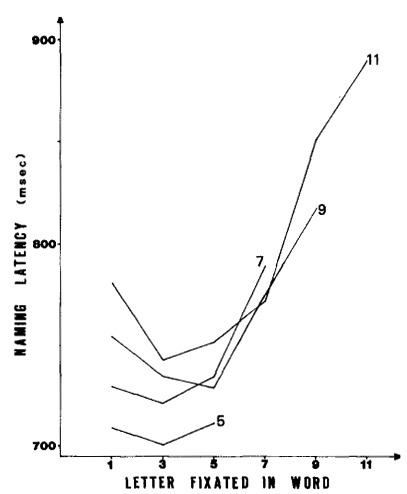
\includegraphics[width=0.4\textwidth]{Pics/ucurve}
\caption{The time it took participants to name the word they saw depending on their fixation point in the word. This graph shows results for words of length 5, 7, 9 and 11. \protect\cite{oregan_convenient_1984}}
\label{fig:ucurve}
\end{figure}

Removing the spacing between words decreases the reading speed with around 30\%. Fixation does not fall on the ORP but tends to the beginning of words. Splitting long words, like long Danish or German compound words, into their individual words, increases reading speed, even though it was grammatically incorrect. Likewise with putting in spaces in Thai, where there are no spaces.

\subsection{Meta-guiding reading (using a pen to keep focus)}
GUSTAV

\subsection{Modes for reading}
BENJAMIN

("gears" - depending on context, you switch "gear"):
Read for memorize
Read for learning
Rauding (sentential integration, lexical + semantic) - most optimal
Skimming (semantic encoding)
Scanning (lexical access? using memory)
Reading rate (WPM) - rauding is the best?
Cognitive speed vs. reading speed
E = AR (E: Efficiency, A: Accuracy, R: Rate)
=======
\subsection{Attention}
MATHIAS

\subsection{Reading Processes}
\citeA{carver_reading_1992} presents five reading processes, also referred to as \textit{gears} (see Figure \ref{fig:trace_cross}). Each gear is defined by its \textit{goal}, \textit{culminating component}, and its \textit{speed}, measured by \textit{WPM} (words per minute). WPM also varies based on reading level, so to block out this bias, \citeauthor{carver_reading_1992} bases his experiments exclusively on college students. The following section is based on his study.

\begin{figure*}[htbp]
\centering
\captionsetup{justification=centering}
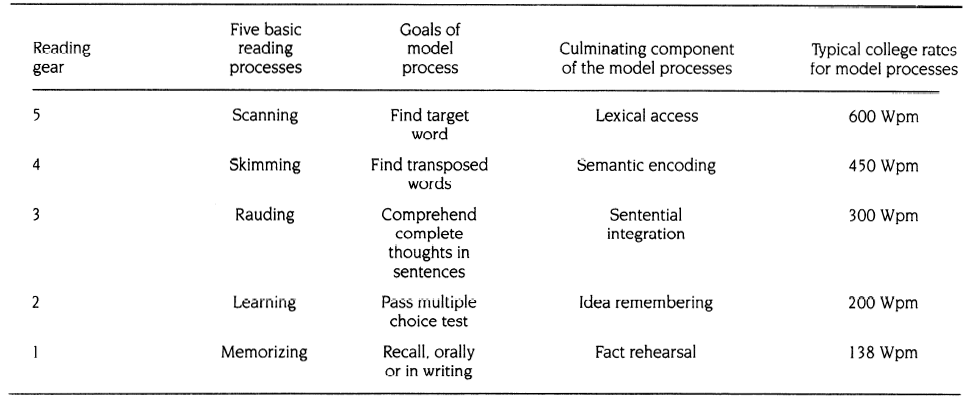
\includegraphics[width=1\textwidth]{Pics/gears_list}
\caption{Each gear has its own goal, culminating component, and WPM. \protect\cite{carver_reading_1992}}
\label{fig:gears_list}
\end{figure*}

The goal relies on the reader's intent when reading the text. For instance, the reader could read the text just to find a single word (scanning). The culminating component of a gear, is then the cognitive process that it requires. \textit{Lexical access} is the component used for finding a single word in memory. If the reader's goal changed to finding a certain sentence in the text, such as in skimming, transposed words must be found and the activity would require an additional component; \textit{semantic encoding}. Other than just finding the words, the reader must now determine the meaning of the sentence. In order for the reader to understand the complete thought of a sentence, the \textit{sentential integration} component must be added. These three components together are the requirement for the most basic and most used reading process - \textit{rauding}, also known as \textit{typical reading}. The word comes from a combination of 'auding' and 'reading', as they both share the same underlying comprehension processes. If the goal of reading the text is to learn, e.g., in order to answer a test, the \textit{idea remembering} component is added. In this gear, some words require re-reading and longer time to process. The final gear is focused around remembering the text and uses the \textit{fact rehearsal} component. This gear requires rehearsing the material and memorizing it. 
\citeA{carver_reading_1992} goes on to mention that the best readers shift up and down in gear while reading, based on the difficulty of the material - a term called \textit{process flexibility}. 

By having college students read a text followed by answering two multiple choice tests, as well as judging their own performance, \citeauthor{carver_reading_1992} tested efficiency at different reading rates. It was found that the students were most efficient at rates around 300 WPM - the rauding reading rate. This rate has therefore been referred to as the most optimal reading rate.
%Efficiency was calculated from the product of accuracy and reading rate, and the accuracy was determined through multiple-choice tests as well as self-judgement.

\citeauthor{carver_reading_1992} also mentions the term \textit{cognitive speed}, which acts as a limit of the reading speed. If the reader passes this limit, he will not be able to operate the culminating components successfully, resulting in a poor comprehension. The main concern however for most students is to make the reading speed reach the limit of the cognitive speed.

\textbf{(Gustav: maybe remove this quote?)}

\citeauthor{carver_reading_1992} describes how the \textit{rauding theory} relates to the \textit{schema theory}. The schema theory uses gears 1 and 2, but mainly focuses on how readers learn or memorize text. \citeA{widmayer_schema_2005} presents schema as a set of rules that help processing new information by interpreting and predicting situations occurring in the environment. Specifically for reading, \citeauthor{widmayer_schema_2005} claims that:

 \emph{''...Correspondingly, teachers of reading have found that activating a learner's schema enables them to better process information that they are reading. Therefore, many advocate teaching learners metacognitive strategies designed to activate one's schema before reading, such as reading heading and the title, looking a visuals in the text, and making predictions based on the title and pictures.''}

This might indicate that when using schema, readers use skimming or scanning before reading a text, but shift to the memorization and learning gears as soon as they start reading. It also indicated that a complete overview of the text can be relevant in some cases.

%(INSERT REF: Reading for One Second, One Minute, or One Year) compares four different theoretical perspectives in reading, each focusing on a certain style and speed of reading: Rauding, Verbal Efficiency, Schema, and Whole Language.

\subsection{Sub-vocalization}
\citeA{bruinsma_should_1980} says that ...
%http://www.jstor.org/stable/20195232
%[Conclusions The evidence cited here should caution teachers to be very careful in their efforts to reduce subvocalization during silent reading. This should be done directly only with students who are otherwise compe tent readers and who are reading relatively easy material ...]

\section{Related Work}\label{relatedWork}
%Camera Path Animator 3.0 (Unity asset store).
%Camera system that follows the character but also focuses on showing the environment - Used in the game God of War.

\begin{figure*}[htbp]
\centering
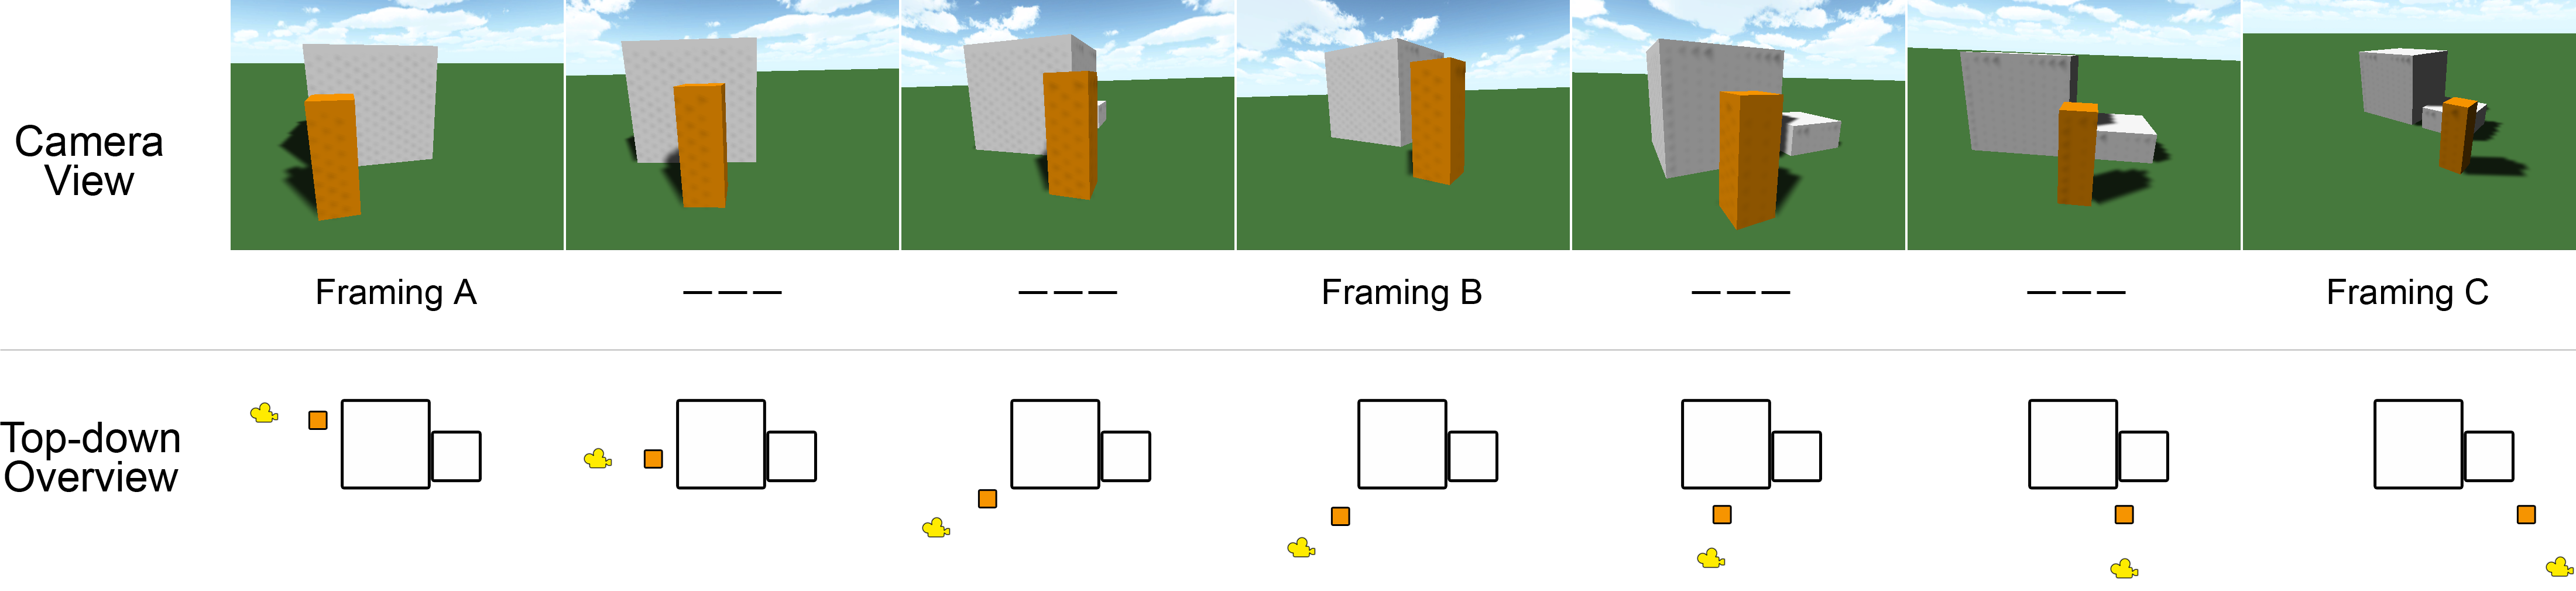
\includegraphics[width=1\textwidth]{Pics/InterpolationExample}
\caption{An example of a camera interpolation between three framings (A, B and C). The framings contain position, rotation and field of view. As the player character (orange cube) moves, the camera follows him by interpolating between the framings.}
\label{fig:InterpolationExample}
\end{figure*}

Automatic camera control is an active research field. In 3D computer animation, a virtual environment is rendered in frames from a specific point of view. This is a complex process that involves technical and artistic tasks, typically requiring the work of several professionals for a long time period \cite{burelli_automatic_2014}. Developing a system that makes the camera animation automatic can be beneficial at both a professional level (to reduce cost) or at an amateur level (to increase quality). Systems that emphasize automatic behaviour have been proposed \cite{bourne_constraintBased_2008, burelli_automatic_2014}; these use an automatic approach for controlling a virtual camera driven by AI techniques. However, the focus of the camera tool proposed in this work is on artistic control. Hence, an automatic approach is not feasible.

In a behind-the-scenes documentary, the developers behind the PlayStation game series \textit{God of War} talk about the importance of being able to frame the scene \cite{gow_camera}. Depending on the context, it is important for them to frame the scene so players know where they should be heading next. They use camera zones to determine what area the player is in and then activate the corresponding camera for that zone. This example shows that it is important that the artists are able to crate framings themselves.

The main requirement of a framing-based camera tool for games is that it can go from one camera setting (A) to another camera setting (B) depending on the player's position or certain events. For instance, A and B can be different in position, rotation and field of view.
%By looking at games with emphasis on its visuals and environments, it was found that the camera changes its position, rotation and field of view. 
Figure \ref{fig:InterpolationExample} shows an example of how the camera interpolates between three positions.

%\begin{figure}[htbp]
%\centering
%
\includegraphics[width=.4\textwidth]{Pics/CameraSystem_BASIC}
%\caption{The camera interpolates between position A and B. A and B contain information about its %position, rotation and field of view.}
%\label{fig:CameraSystem_BASIC}
%\end{figure}

%\subsection{Camera Tools}
The tool Camera Path Animator \cite{unity_camTool} can be used for creating animated cameras within the game engine Unity \cite{unity_main}. As the name suggests, it works by animating the camera along a specified path, which can have various shapes (e.g., Bezier and Hermite curves). The tool is primarily targeted towards creating cameras that move linearly along a set path, i.e., for use in cinematic sequences. It provides various ways of inserting, moving and deleting points, as well as changing settings such as field of view, speed, interpolation type and easing. Additionally, it has an event system for triggering certain events at certain points in the path. For our tool, it was important that the artists can create framings themselves and that the interface in general is designed for the artists; hence, we chose not to extend the Camera Path Animator, but instead took inspiration from it.

%Why we don't use Camera Path Animator:
%Customizable interface
%Specific for artists
%Freedom
%Flexibility
%Maya knowledge
%Path

%\begin{figure}[htbp]
%\centering
%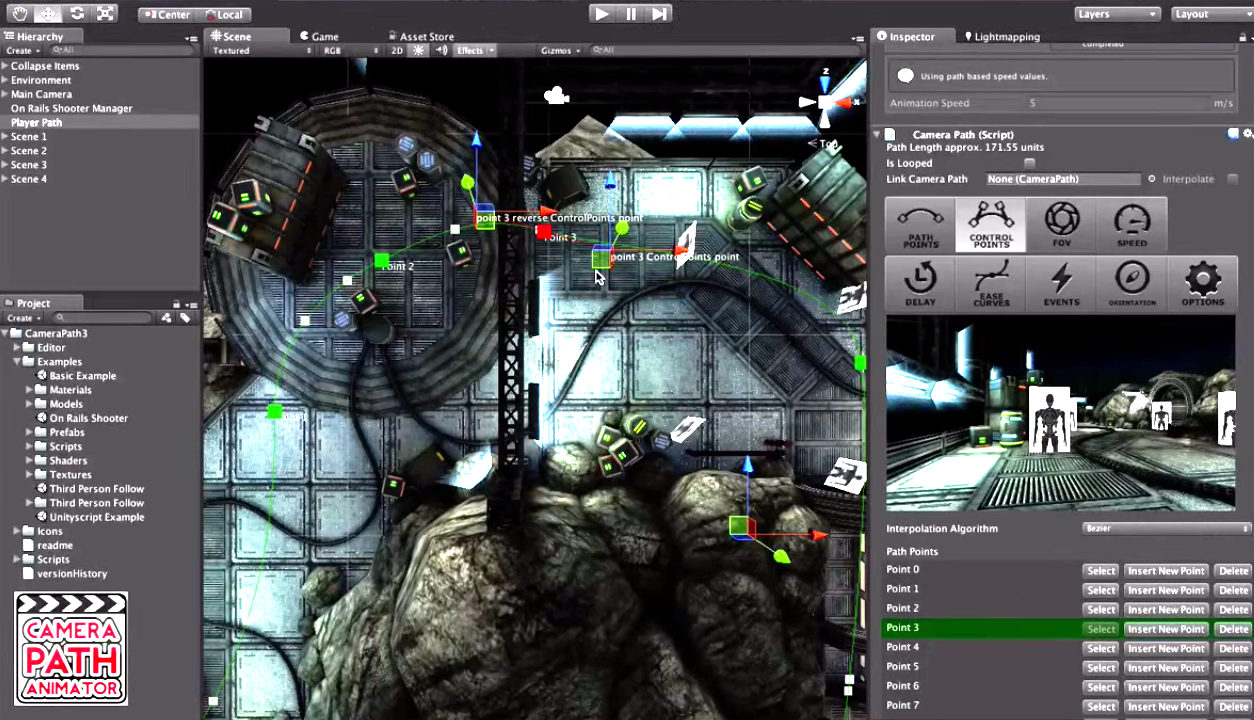
\includegraphics[width=0.40\textwidth]{Pics/unity_path_cam_tool}
%\caption{Overview of the objects related to the camera system.}
%\label{fig:unity_path_cam_tool}
%\end{figure}

%The God of War video game franchise for the PlayStation systems has also made notable use of their camera systems. The developers call the system Rail Driven Cameras and consists of a 'rail' that will be placed in the game world. A camera is keyed in both ends of the rail, and the camera will then animate between them as the protagonist moves along the rail. % Det her føles pølse, ikke meget at skrive om det og super unscientific

%\begin{figure}[htbp]
%\centering
%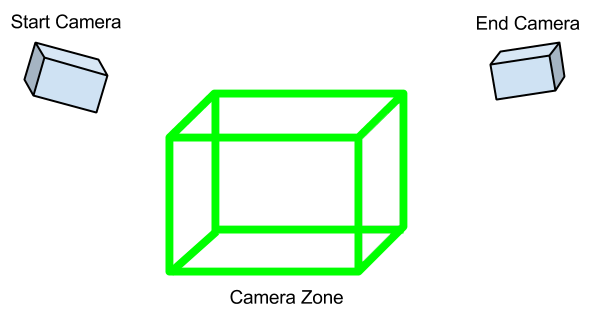
\includegraphics[width=0.45\textwidth]{Pics/gow_cameraZones2}
%\caption{When the player enters a camera zone, the camera will interpolate between the two pre-%defined cameras associated with that zone.}
%\lab%el{fig:gow_zones}
%\end{figure}

%\begin{figure}[htbp]
%\centering
%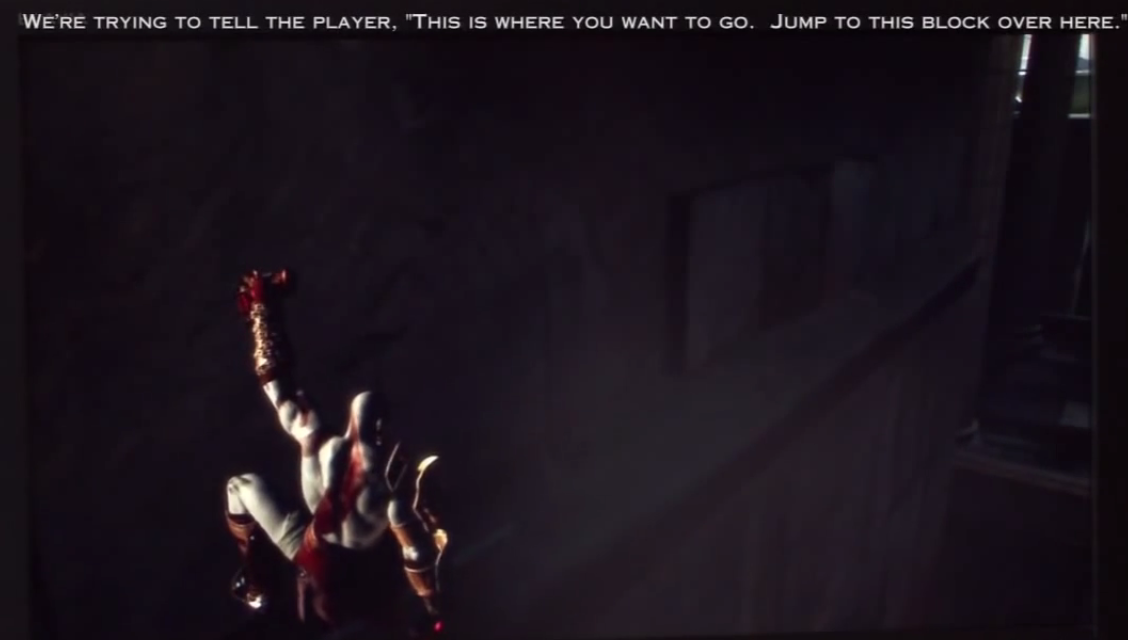
\includegraphics[width=0.40\textwidth]{Pics/gow_next}
%\caption{The camera's framing can help the designer guide the player in the right direction.}
%\label{fig:gow_jump}
%\end{figure}


%An example of this is when the main character has to jump from one 



%\textbf{Scientific material: Write about automatic camera tools (Paulo something-something) - even though we are not using it. Make it clear that our work is different from how other people's camera tools work}

%\subsection{Participatory Design}
Participatory design has been defined as the participation of users in the design process of a system that is to be implemented in an organization \cite{kensing_participatory_1998}. By involving users in the design, their skills, experiences, and interests are taken into consideration, thereby increasing the likelihood that the system will be useful to them.

According to participatory design researchers, it is important that there is an active cooperation between the designer and the user \cite{kensing_participatory_1998}. This results in the designer gaining knowledge of the user's current work practices, and the user gaining knowledge of the technology being developed. It is also important that users take an active part in the analysis of needs, selection of technology, design and prototyping, as well as organizational implementation.
\section{Preliminary Study}
We did bla bla bla ...

\subsection{Participants}
	Interviews (Knapnok Games, Unity Studios)
	Online questionnaires (27 game developers)
	Observations (4-5 students at TAW)
	
	The interview sessions involved a total of three people from two game studios in Denmark; Project Lead at Knapnok Games in Copenhagen and Lead Designer and Lead Programmer at Unity Studios in Aarhus.
The online questionnaire received 27 submissions from people with a median professional experience of 3 years (SD 2.67).
Lastly, the participatory paper prototyping was done on 4 students at TAW. (from the team?!)

	
\subsection{Methods}
		Interview design (semi-structured)
		Questionnaire design
		Observations (from meetings, discussions)
		Paper prototyping
		Participatory design
		
		The interviews were conducted at the respective companie' offices using a semi-structured approach. The interviews was audio recorded and notes were taken during the interview. We were offered to see the tools they use in production in practice. The session at KnapNok Games took one hour and two hours at Unity Studios.
The questionnaires was published on relevant game development communities. (unity forum, tigsource, 3Dboss.com, game dev facebook groups and twitter). The questions in the questionnaire and the semi-structured interview was designed to be case-specific (hendrik bog) in hope of gathering more detailed information. Both the interviews and questionnaire was analysed with using grounded theory
The paper prototyping was a participatory design - dialogue-based prototyping session. The participants wrote down their requirements while thinking aloud. They then designed their "dream interface" using paper blocks. They expressed their decisions and ideas while doing so. A facilitator would ask why they needed certain elements and why it was chosen to structure it as they did.


\subsection{Findings}
	Frequently mentioned points
	
	The two game studios that were interviewed both use Unity in their development and mentioned that it is most efficient if everyone on the development team is able to use Unity. This allows team members non-programmers (e.g. artists and designers) to implement assets themselves as well as tweak parameters and build functionality using tools made by the programmers. This way, the amount of interactions between programmers and non-programmers are minimized, and non-programmers can take on more tasks.
Among the tools made for non-programmers was 
Points derived from the questionnaire mentions the more tweakable  your design is, the better, i.e. changing variables without going into the code in a text editor. However, this can also be of nuisance as the number of accessible variables can confuse them. A tool also have to be presented clearly. Finally it is important that the designers know the tools they are working with.
During the paper prototyping, the participants continuously mentioned Maya (the software package they're most accustomed to) when trying to explain how they had envisioned the camera tool working; they wanted something close to Maya.

\section{Participatory Design}
An initial mockup of the tool's interface and functionality was created internally. The mockup had the interface all gathered in one window to keep the design minimalist. However, in search of a better design, we included the end-users in the process going forward (see Figure \ref{fig:mockup}).

To ground our design work, we were interested in learning more about our users and how they envisioned the finished product. Therefore, three participatory exercises were conducted \footnote{The exercises were video documented, except for one artist and half of the footage from another artist in the first exercise}. The first of which was done to know their general workflow when working with cameras in the tools they, namely Maya and Unity. Secondly, we wanted to know which features they requested and how they envisioned the finished tool. Finally, they tried using a prototype of the camera tool based on their initial design and feature requests.


\begin{figure}[htbp]
\centering
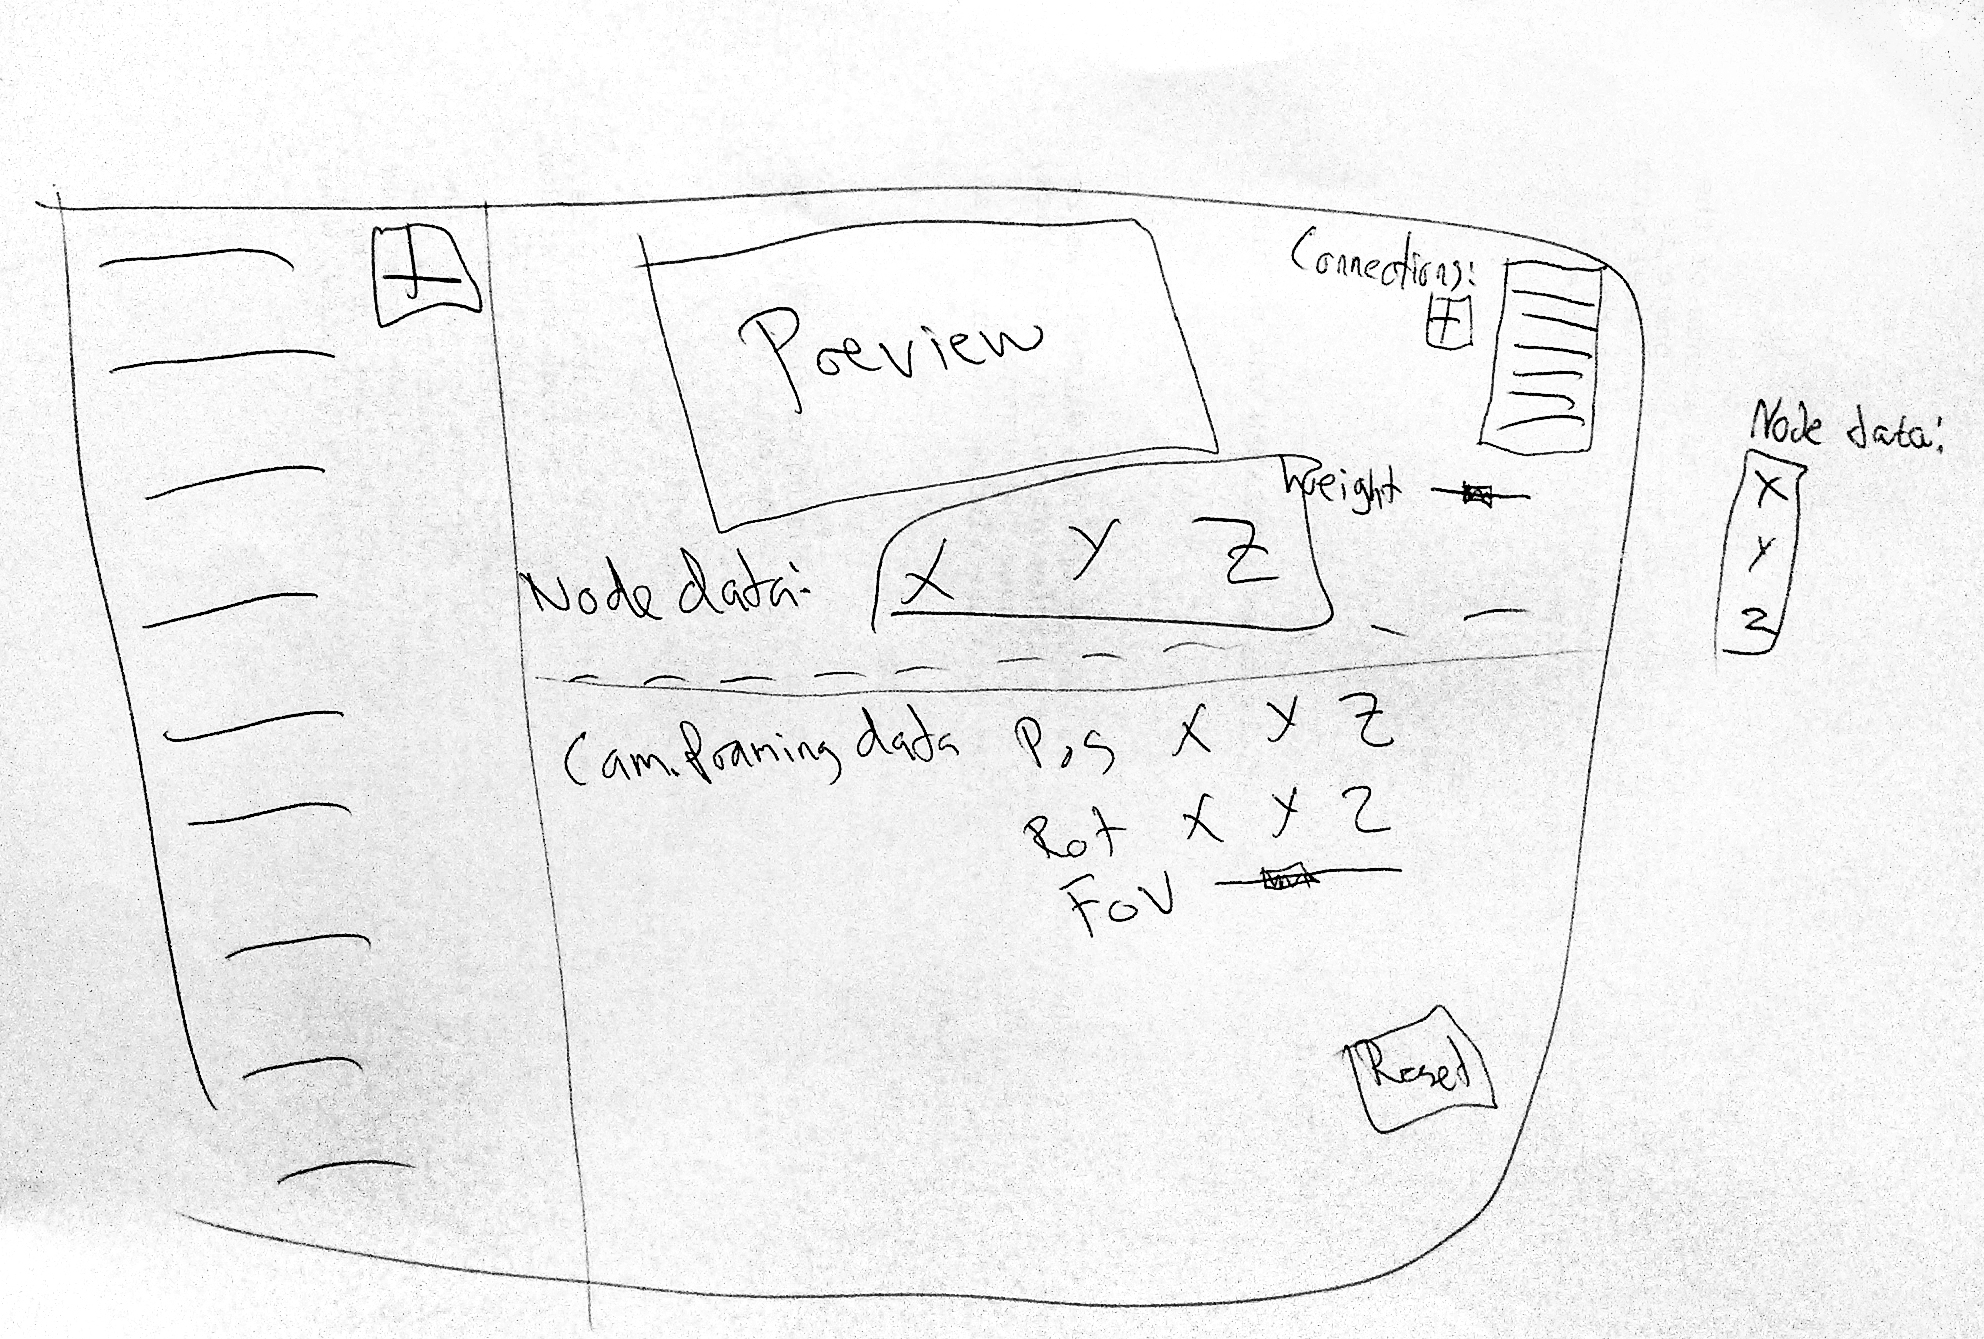
\includegraphics[width=0.50\textwidth]{Pics/InitialMockup}
\caption{The initial concept was to have all the feature tools inside one big window. Early on it was observed that all of the students from The Animation Workshop use a dual-monitor setup, they could then dedicate one monitor to the camera tool.}
\label{fig:mockup}
\end{figure}

\subsection{Exercise 1: Knowledge of tools} \label{exerciseOne}
An artist and a facilitator sat down in front of the artist's work area. The facilitator then asked the artist to show him how he would animate a camera around an object in Maya (see Figure \ref{fig:mads_dual}). This included keyframing and how to change the camera settings for each keyframe. This was done to get an idea of how they usually work. If our camera tool should be successful at helping these artists, it should mimic some of the same behaviour that Maya has. It seemed ideal that the users should be able to utilize their previously-gained knowledge from Maya wherever applicable.

\begin{figure}[htbp]
\centering
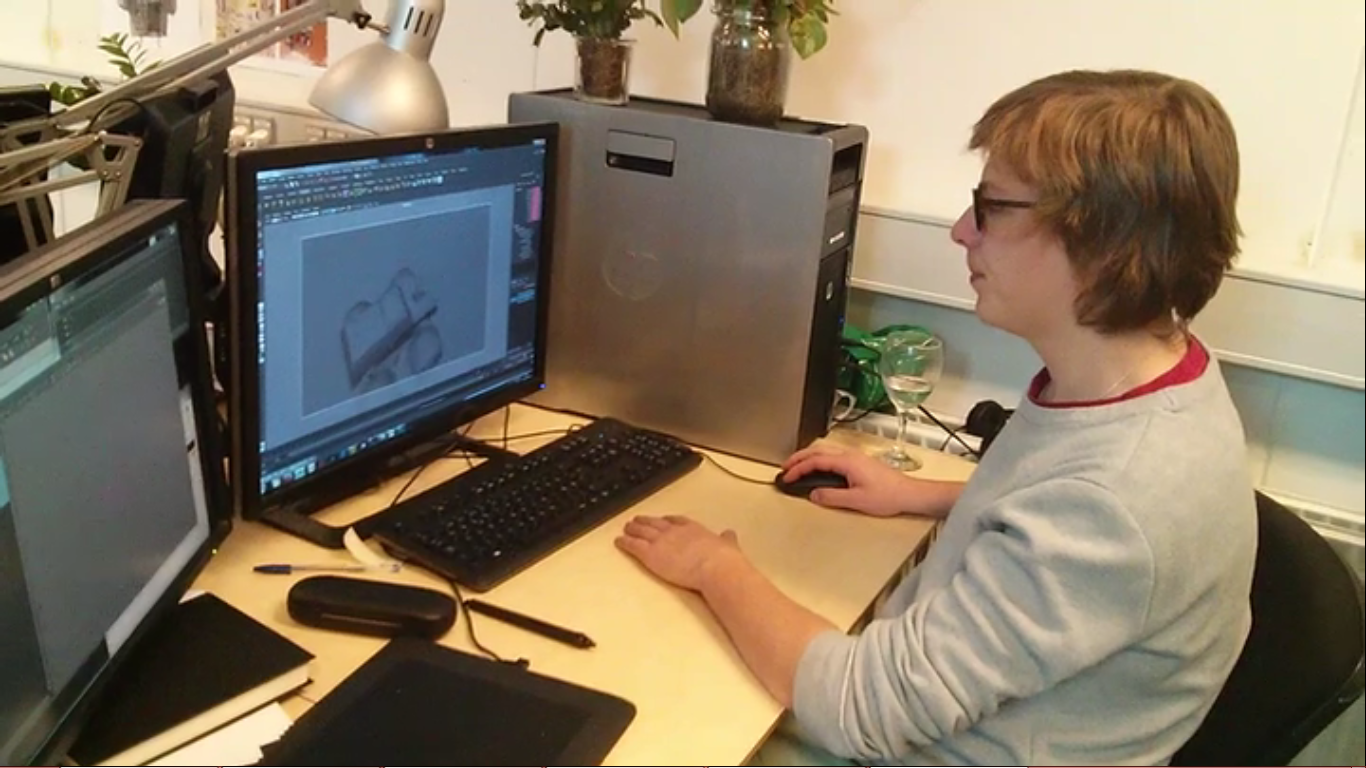
\includegraphics[width=0.50\textwidth]{Pics/Mads_dual}
\caption{All the students at The Animation Workshop work with a dual monitor setup.}
\label{fig:mads_dual}
\end{figure}

After this, the facilitator and artist switched to Unity where he was tasked with moving around in the scene and then to create basic objects such as cubes and spheres, as well as positioning the camera. The purpose of this was to get an understanding of how skilled they are at using Unity - moving around the scene, rotating and translating objects etc. This was done with another two artists as well. The first section of the exercise, the Maya part, was the same for all three artists, but the questions and tasks changed in the last section as the facilitator gained new knowledge about their skill level.

It was discovered that none of the artists knew how to use a standard Unity feature that lets the player fly around with the scene camera as if they were playing a first-person game ("Flythrough Mode", \cite{unity_flyMode}). The artist were excited about the discovery of this feature. One artist perceived the standard way of moving around in Unity as confusing, while another stated that the way of moving the camera is exactly like in Maya. After testing this ourselves, we concluded that the movement controls in Maya and Unity are indeed very similar (except for the "Flythrough Mode"), which means that the artists should ideally be comfortable with navigating in either of the applications.

\subsection{Exercise 2: Feature list and paper prototyping}
The artists were given a blank sheet of paper and a pen and was tasked to draw and write about the camera tool, as they envisioned it in a free-form approach. They then explained what they did and they had a discussion about it. There were no strict requirements of how they approached the task, so some focused a lot on feature requires, while others were more interested in fundamental workflow and user interfaces. This was done with four artists in total.

After this, the same four artists were placed at a desk, one by one, where a variety of labels were laid out in front of them (see Figure \ref{fig:labels}). These labels were marked as different sliders, buttons, windows, field parameters, camera settings, etc. The labels were primarily based on the basic building blocks of Unity's user interface, as well as some of the observations from the first exercise where the users talked about how they worked with Maya.


\begin{figure}[htbp]
\centering
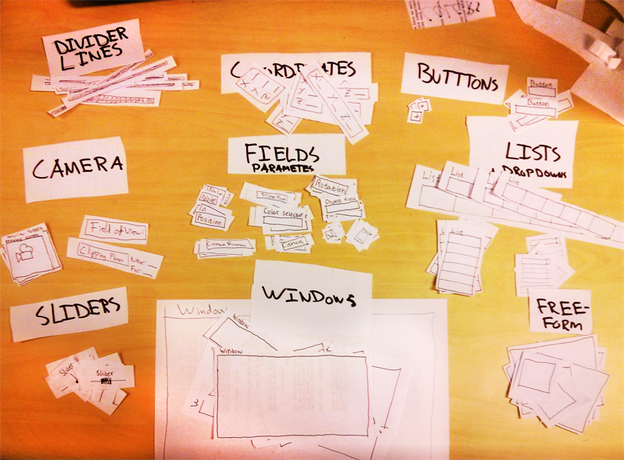
\includegraphics[width=0.50\textwidth]{Pics/labels}
\caption{The users were asked to design their "dream program" by using paper labels as building blocks. They were also allowed to draw their own components if necessary.}
\label{fig:labels}
\end{figure}


All artists wanted basic features like translation, rotation, field of view of the camera, as well as a curve editor to change the interpolation between two cameras. After these features, all the artists diverted in their designs. All the designs were discussed internally and main points and ideas were extracted from them. These findings were used as the foundation of the tool's design. However, the foundation for the program was not strictly based on the artists ideas and requirements; instead, we tried to extract some more general requests of what they as artists actually need. It was important to keep in mind that working in an interactive medium such as game development was a new experience for the users.

A slider that could be used to interpolate between two camera framings in a preview window is an example of an idea that was discarded by us. The artist wanted two preview windows of the camera framing, as well as a preview window of the interpolation, which the slider would manipulate. His idea was similar to a DJ turntable. After discussing it internally, we concluded that this idea would make the interface too elaborate, but the idea of being able to preview your changes quickly was kept.

See Figures \ref{fig:morten_requirements} and \ref{fig:mads_turntable}.

% morten
\begin{figure}[htbp]
\centering
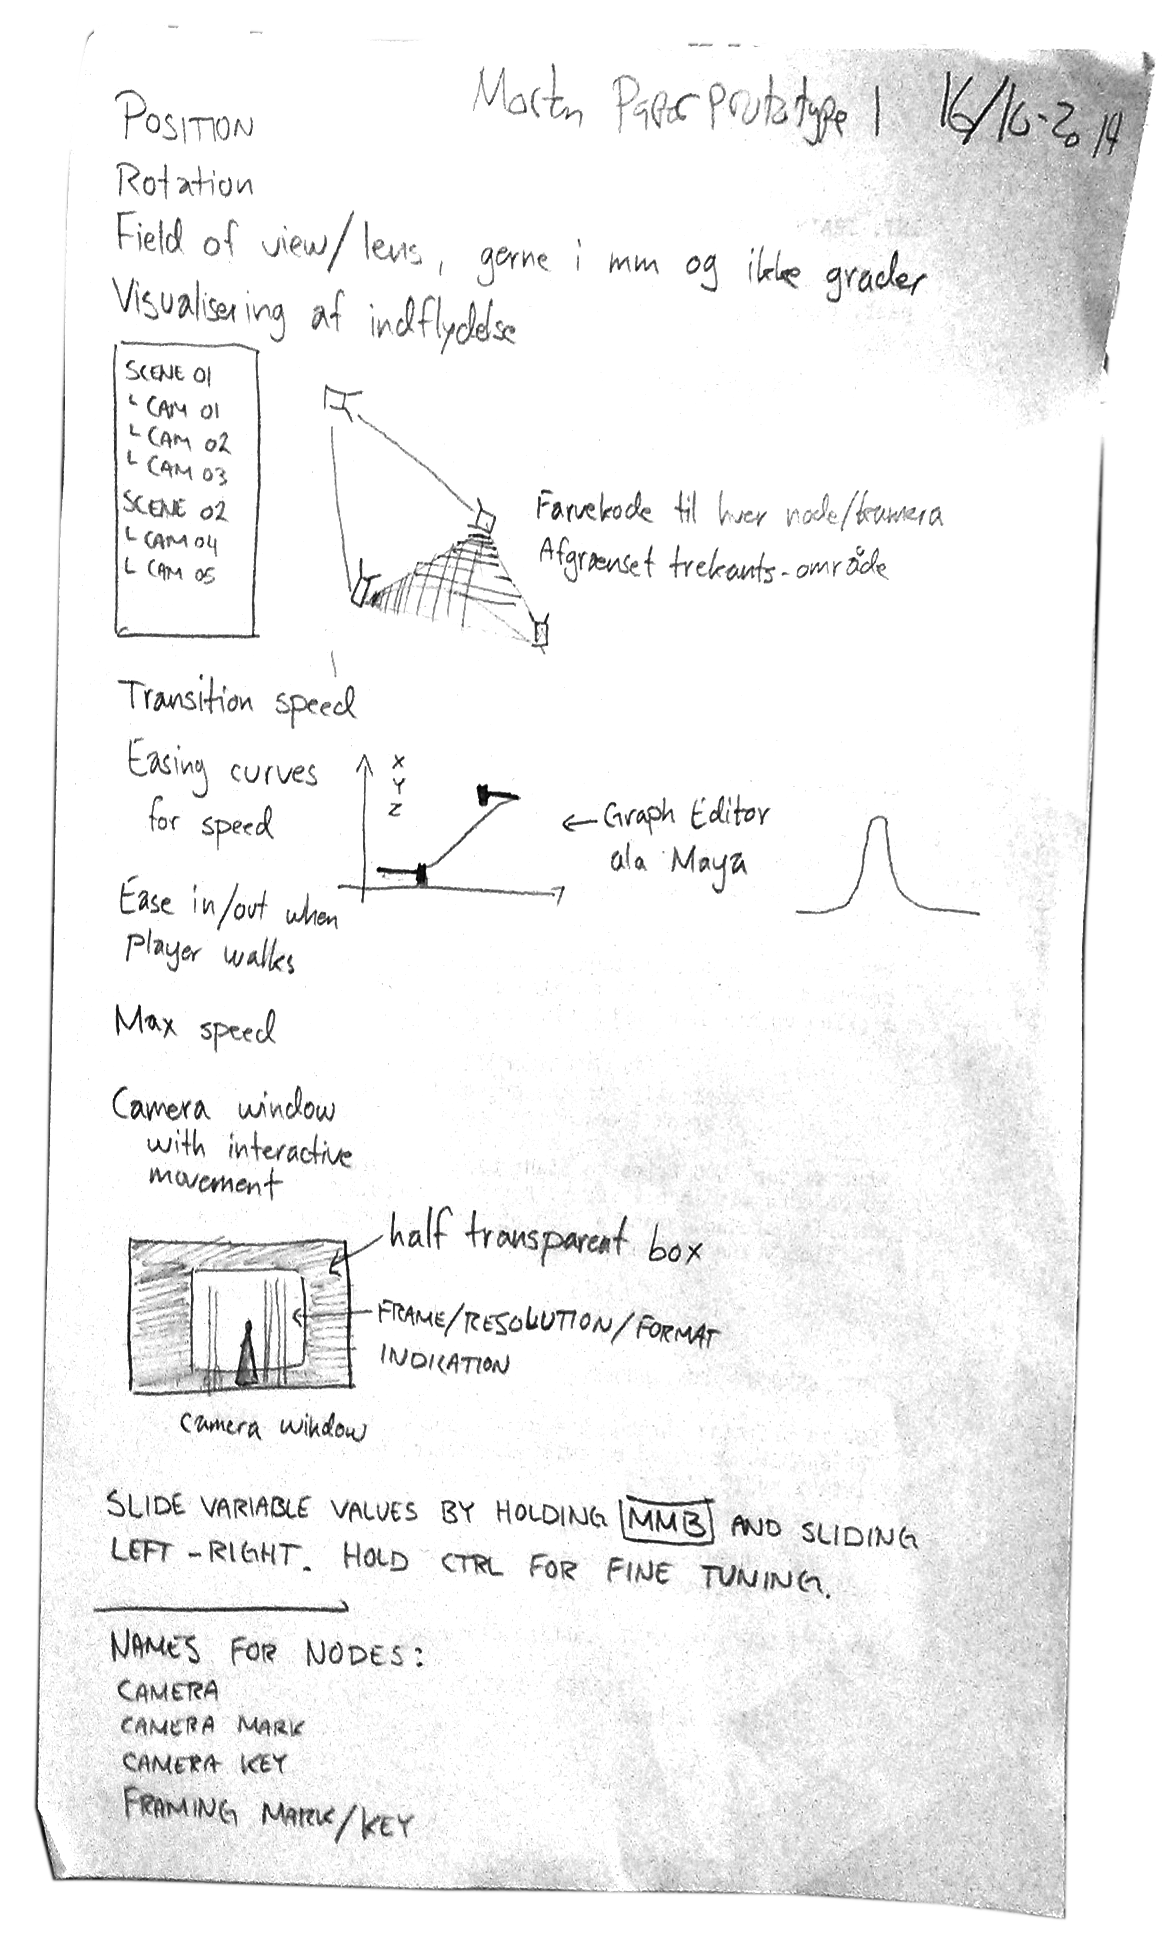
\includegraphics[width=0.50\textwidth]{Pics/Morten01}
\caption{Feature requirements.}
\label{fig:morten_requirements}
\end{figure}

% mads
\begin{figure}[htbp]
\centering
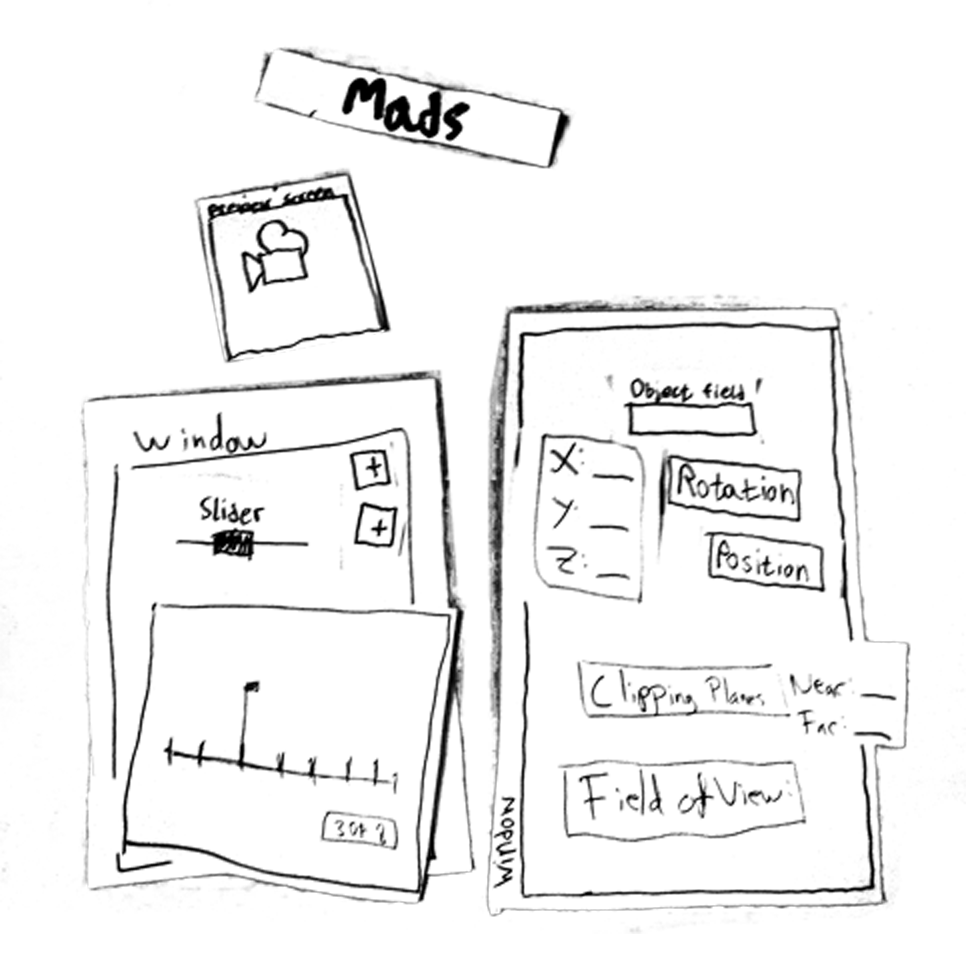
\includegraphics[width=0.50\textwidth]{Pics/Mads01}
\caption{Turntable concept.}
\label{fig:mads_turntable}
\end{figure}

\subsection{Summary of Findings}
\begin{itemize}
\item Basic translation and rotation
\item Field of View
\item Camera modes
\item Domains/areas/trigger zones
\item Toggle camera to either follow or be static
\item Curves and graph editors
\item Quick real-time preview
\item Have triangle in UI that represents the three cameras. Have a 'object' inside that you can manipulate to change the preview (like yellow man in Google Maps)
\item Camera lenses and effects (fish-eye, etc.)
\item Use "aim point" to place the camera
\item "Be the camera" when positioning it
\item Easing (maybe presets?)
\item Hotkey to set new camera mark ("S")
\item Different controls modifiers 
\item Hold shift/ctrl/alt to decrease/increase increment / step size
\item Color code the camera keys/markers
\item Use preview screen as separate window to put on secondary monitor
\item 2D overview of the map with all camera keys/markers
\item When looking through the camera, have transparent border (like in Maya)
\item In camera preview, show what camera is currently 'dominant' (how much weight each camera is pulling)
\item Separate windows that can be docked
\item Allows for multi screen setup
\end{itemize}

\subsection{Exercise 3: First iteration}
After having completed the two exercises, we started developing a rough prototype in Unity (see Figure \ref{fig:prototype}). This iteration included basic functionality to make it possible to test and get feedback as quickly as possible. During one of their daily SCRUM meetings, we presented the tool, as well as providing them a short manual (SEE APPENDIX A).


\begin{figure}[htbp]
\centering
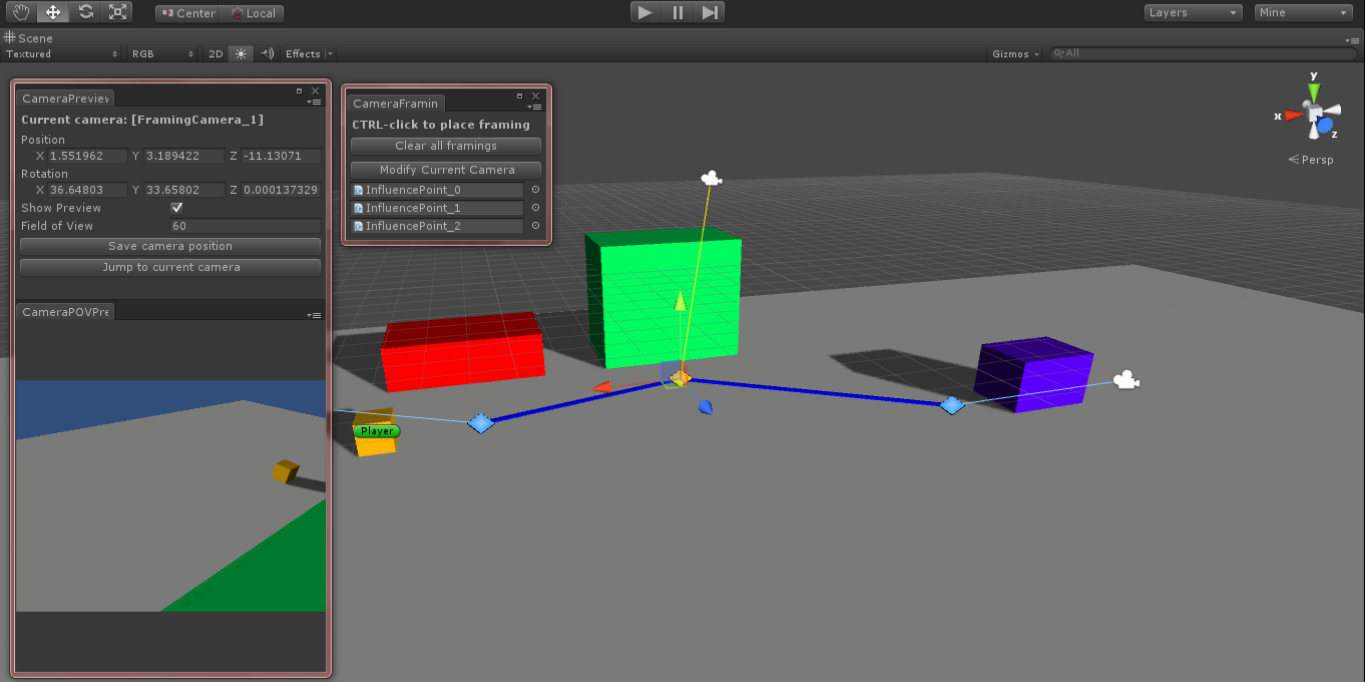
\includegraphics[width=0.50\textwidth]{Pics/MainSetup}
\caption{Rough prototype with basic camera manipulation.}
\label{fig:prototype}
\end{figure}

Three artists tried it out for 10-40 minutes each. They got a chance to try out the tool, as well as expressing their overall opinion about how they preferred the workflow to be.


The facilitator gave the artist small tasks like “Can you place Framings along this paths?” and “Can you try and set the Framing’s camera settings as you’d like?”. This exercise was semi-structured, and not all questions were predetermined; some was thought up as the exercise went on.

Over the course of the exercise, some key points was discovered through observation or discussion with the artist. The biggest piece of feedback revolved how the users are supposed to place the virtual camera in the scene. Initially, users were supposed to use Unity’s "Flythrough Mode" (see Section \ref{exerciseOne}) and place the camera as they liked. Then, they should press the "Save camera position" button (see Figure \ref{fig:prototype}). However, some users were confused about this, since they thought that they now they continuously looked through the camera's point of view, i.e. if they moved around after they'd pressed the button, the framing camera should be changed as well. This was not how the system worked, since it simply just saved the scene camera's position to the framing camera whenever the button was pressed. In other words, the users mental models didn't fit with how the tool worked.

\section{Experiment}
%Give artists the task to make a video in a certain scene using some specific features, both in Unity and in Maya. We can then compare their performances, and if the two performances are significantly close, the tool was a success.

%Video and audio recordings. Time spent on tasks. Few questions about usability and experience.

%(Hypotheses - not sure yet?)

\subsection{Purpose of the test}
\begin{enumerate}
\item To find out if the FEELS team’s mental models of the camera system match how the system actually works.
\item Compare other artists from TAW 3rd year using the camera system with the FEELS team.
\end{enumerate}


%Figure \ref{fig:test_overview} shows the criteria for the two testing groups \footnote{This will not be in the final paper; it's just for helping you to understand what we mean.}


%\begin{figure}[htbp]
%\centering
%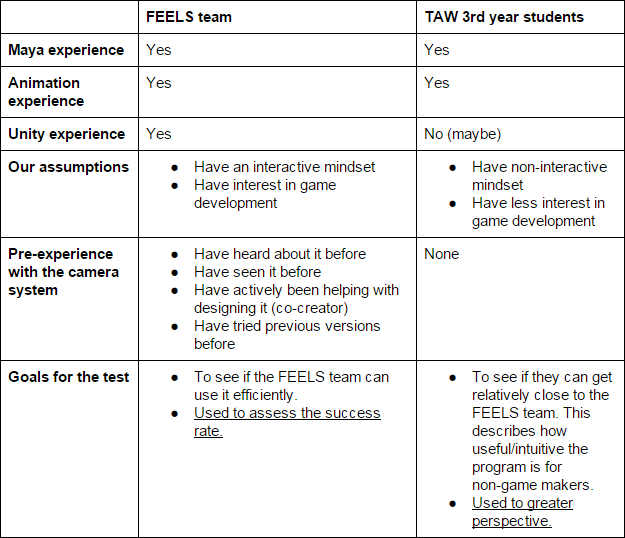
\includegraphics[width=0.5\textwidth]{Pics/test_table_temp}
%\caption{Overview of the testing groups.}
%\label{fig:test_overview}
%\end{figure}

\subsection{The Three Phases of the Experiment}
\textbf{PHASE 1 - Training:}
\begin{enumerate}
\item Place framings along the movement path so that there's at least one framing in "move path section".
\item Tell the facilitator about the functionality of each button in the interface as you think it'll work.
\item Split a framing connection into two.
\item Delete a framing.
\end{enumerate}

Specific tasks:
\begin{enumerate}
\item Make the camera's field of view change when player gets close to it
\item Make the camera tilt upwards when player gets close to it
\item Make the camera pan to the left when player gets close to it
\item Make the camera look at object X when the player gets close to it
\item Make the camera dolly away from the character as the player walks along a path.
\item Make the camera look from the ground upwards
\item Change the interpolation of one of the previous assignments by changing the animation curve.
\end{enumerate}

\textbf{PHASE 2 - Re-create camera:}
\begin{itemize}
\item Show a video of the end result
\item Recreate this as closely as possible?
\end{itemize}

\textbf{PHASE 3 - Be creative:}
\begin{itemize}
\item Give them environment with path already there, do what you want. Test the limits of the system.
\end{itemize}

\section{Results}
Our results ...
\section{Conclusion}
We found that ...
\section{Discussion}
\subsection{Principles and Guidelines}
General findings that can be learned from this study. Could be something like the "180 degree rule" of games. Examples: that the barycentric interpolation works better than triangulation; that you should at maximum have four cameras; that cutting between multiple cameras confuses the player if the cutting speed is less than X, etc. In short, something the reader can use after having read the paper.

%%% ---------- How to make headlines and sections ---------- %%%
\section{This is a section} \label{sec:thisSection}
\subsection{This is a subsection}
Let us refer to section \ref{sec:thisSection}.

%%% How to write bold, italics %%%
This text is \textbf{bold}.
This text is \textit{italics}.

%%% ---------- Insert page break ---------- %%%
%%\newpage
%%Here is some text on the next page

%%% ---------- This is how you refer to a figure in the text ---------- %%%
Here is something that I illustrate in figure \ref{fig:wavelength}.

%%% ---------- This is how you insert a single picture ---------- %%%
\begin{figure}[htbp]
\centering
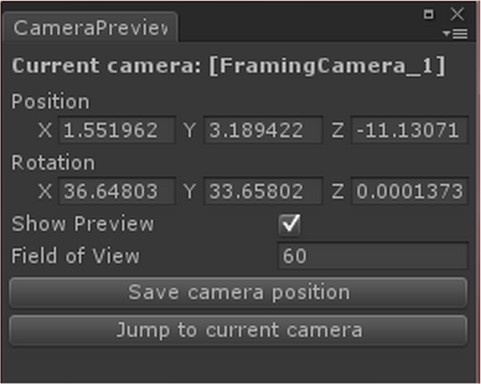
\includegraphics[width=0.50\textwidth]{Pics/Dummy}
\caption{Image caption text goes here bla bla bla bla}
\label{fig:wavelength}
\end{figure}

%%% ---------- This is how you insert multiple pictures ---------- %%%
\begin{figure}[htbp] \centering
\begin{minipage}[b]{0.45\textwidth} \centering
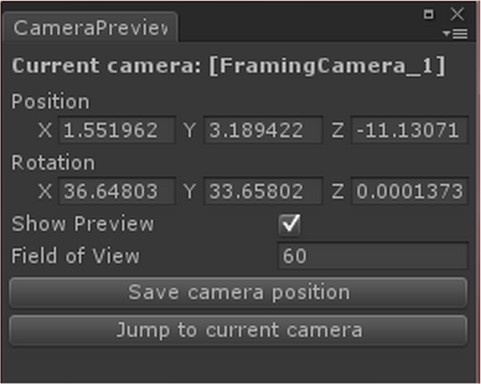
\includegraphics[width=0.60\textwidth]{Pics/Dummy} % Venstre billede
\end{minipage} \hfill
\begin{minipage}[b]{0.45\textwidth} \centering
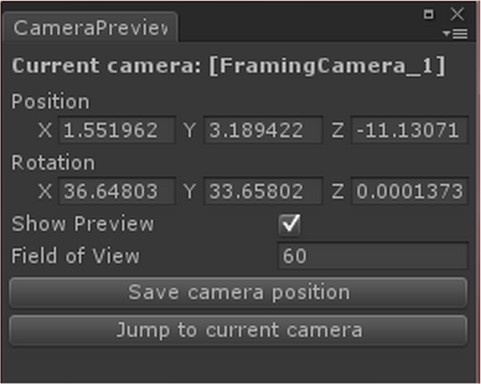
\includegraphics[width=0.60\textwidth]{Pics/Dummy} % Højre billede
\end{minipage} \\ % Captions og labels
\begin{minipage}[t]{0.45\textwidth}
\caption{Caption text for left picture.} % Venstre caption og label
\label{fig:cap1}
\end{minipage} \hfill
\begin{minipage}[t]{0.45\textwidth}
\caption{Caption text for right picture} % Højre caption og label
\label{fig:cap2}
\end{minipage}
\end{figure}

%%% ---------- This is how to make a source reference ---------- %%%
According to bla bla \cite{haigh-hutchinson_real-time_2009} %% passive source
at cite flere: \cite{haigh-hutchinson_real-time_2009, haigh-hutchinson_real-time_2009, haigh-hutchinson_real-time_2009}


%%% ---------- This is how to make bullet points ---------- %%%
\begin{itemize}
\item \textbf{Wavelenght} - Measured in meters from wave top to wave top and denoted as $\lambda$.
\item \textbf{Frequency} - Measured in oscillations per second, Hz, denoted $f$.
\item \textbf{Energy} - Measured in electronvolts, eV, denoted $E$.
\end{itemize}

%%% ---------- This is how to do math stuff ---------- %%%
To derive the wavelength or the frequency, formula \ref{eq:wavelenght} is applied:
\begin{align}
\centering 
\lambda = \frac{C}{f}
\label{eq:wavelenght} 
\end{align}
where {$C$} is the speed of light.



%%% This is how to make footnotes %%%
Hello, I need a footnote \footnote[0]{You can read me, no?}.

%%% This is how to insert a table %%%
\begin{table}[htbp]
\centering
\begin{tabular}{|l|c|c|}
\hline
& Personer
& Totalpris \\\hline
Lasagne
& 4
& 160
\\\hline
Flødekartofler
& 6
& 210
\\\hline
\end{tabular}
\caption{Valg af mad.}
\label{tab:mums}
\end{table} %% GUSTAV'S GUIDE: look at this for how to insert figures, quotes, etc.

%% BONUS STUFF WE MIGHT NEED TO LOOK AT LATER ---------------- VVVVV

%ACKNOWLEDGMENTS are optional
%\section{Acknowledgments}
%This section is optional; it is a location for you
%to acknowledge grants, funding, editing assistance and
%what have you.  In the present case, for example, the
%authors would like to thank Gerald Murray of ACM for
%his help in codifying this \textit{Author's Guide}
%and the \textbf{.cls} and \textbf{.tex} files that it describes.

%
% The following two commands are all you need in the
% initial runs of your .tex file to
% produce the bibliography for the citations in your paper.
\bibliographystyle{abbrv}
\bibliography{references}  % sigproc.bib is the name of the Bibliography in this case
% You must have a proper ".bib" file
%  and remember to run:
% latex bibtex latex latex
% to resolve all references
%
% ACM needs 'a single self-contained file'!
%
%APPENDICES are optional
%\balancecolumns
%\appendix
%Appendix A
%\section{Headings in Appendices}
%The rules about hierarchical headings discussed above for
%the body of the article are different in the appendices.
%In the \textbf{appendix} environment, the command
%\textbf{section} is used to
%indicate the start of each Appendix, with alphabetic order
%designation (i.e. the first is A, the second B, etc.) and
%a title (if you include one).  So, if you need
%hierarchical structure
%\textit{within} an Appendix, start with \textbf{subsection} as the
%highest level. Here is an outline of the body of this
%document in Appendix-appropriate form:
%\subsection{Introduction}
%\subsection{The Body of the Paper}
%\subsubsection{Type Changes and  Special Characters}
%\subsubsection{Math Equations}
%\paragraph{Inline (In-text) Equations}
%\paragraph{Display Equations}
%\subsubsection{Citations}
%\subsubsection{Tables}
%\subsubsection{Figures}
%\subsubsection{Theorem-like Constructs}
%\subsubsection*{A Caveat for the \TeX\ Expert}
%\subsection{Conclusions}
%\subsection{Acknowledgments}
%\subsection{Additional Authors}
%This section is inserted by \LaTeX; you do not insert it.
%You just add the names and information in the
%\texttt{{\char'134}additionalauthors} command at the start
%of the document.
%\subsection{References}
%Generated by bibtex from your ~.bib file.  Run latex,
%then bibtex, then latex twice (to resolve references)
%to create the ~.bbl file.  Insert that ~.bbl file into
%the .tex source file and comment out
%the command \texttt{{\char'134}thebibliography}.
% This next section command marks the start of
% Appendix B, and does not continue the present hierarchy
%\section{More Help for the Hardy}
%The acm\_proc\_article-sp document class file itself is chock-full of succinct
%and helpful comments.  If you consider yourself a moderately
%experienced to expert user of \LaTeX, you may find reading
%it useful but please remember not to change it.
\balancecolumns
% That's all folks!
\end{document}
